
\documentclass[11pt,a4paper]{CLabBookTemplate} %load the style file for the Extended Essay

\addbibresource{MyBibliography.bib} %specifying the bibliography file

% information about you and the document
\author{Tim Meiwald}
 %000017-0104 -> candidate number
\usepackage{multicol}


% For the C code snippets
\usepackage{listings}
\usepackage{xcolor}
\usepackage{mhchem}

\definecolor{mGreen}{rgb}{0,0.6,0}
\definecolor{mGray}{rgb}{0.5,0.5,0.5}
\definecolor{mPurple}{rgb}{0.58,0,0.82}
\definecolor{backgroundColour}{rgb}{0.95,0.95,0.92}

\lstdefinestyle{CStyle}{
	backgroundcolor=\color{backgroundColour},   
	commentstyle=\color{mGreen},
	keywordstyle=\color{magenta},
	numberstyle=\tiny\color{mGray},
	stringstyle=\color{mPurple},
	basicstyle=\footnotesize,
	breakatwhitespace=false,         
	breaklines=true,                 
	captionpos=b,                    
	keepspaces=true,                 
	numbers=left,                    
	numbersep=5pt,                  
	showspaces=false,                
	showstringspaces=false,
	showtabs=false,                  
	tabsize=2,
	language=C
}

\lstdefinestyle{PythonStyle}{
	backgroundcolor=\color{backgroundColour},   
	commentstyle=\color{red},
	keywordstyle=\color{blue},
	numberstyle=\tiny\color{mGray},
	stringstyle=\color{mGreen},
	basicstyle=\footnotesize,
	breakatwhitespace=false,         
	breaklines=true,                 
	captionpos=b,                    
	keepspaces=true,                 
	numbers=left,                    
	numbersep=5pt,                  
	showspaces=false,                
	showstringspaces=false,
	showtabs=false,                  
	tabsize=2,
	language=Python
}

\lstset{language=C}




\title{MA4080 - Computational Task 2 } % use capitals


% \component{Electronic Lab Book} % or Lab report, Exploration, etc
% \session{Year 1 Semester 1}

% \wordcount{xxxx} %change this to the actual number

\usepackage{graphicx}

\begin{document}

\pagenumbering{roman} %roman page numbers to be used on the title, abstract, acknowledgment and contents page
\setcounter{page}{1} % start with page 1

\maketitle % generating the title page




% Generating the table of contents
\thispagestyle{fancy} % put the required information in the header
\addcontentsline{toc}{section}{Contents} % include this in the table of contents
\mytableofcontents
\newpage % Start the main text on a new page


% Here comes the important part, the main text
\pagenumbering{arabic} % arabic page numbers to be used from now on
\setcounter{page}{1} % start again with page 1

\section{Classic Endemic Model}
\subsection{Theory and Analysis}
\begin{gather}
	\textrm{Classic Endemic Model Equations} \notag \\	
	\label{Eq:CEM1}
	\frac{ds}{dt} = -\beta is + \mu - \mu s, \; s(0) = s_{0} \geq 0 \\
	\label{Eq:CEM2}
	\frac{di}{dt} = \beta is - (\gamma + \mu)i, \; i(0) = i_{0} \geq 0
\end{gather}
Where $\beta$ is the contact rate of each person in a population.\\
$\mu$ is a factor that affects both births and deaths depending on what it's multiplied by. Where the mean lifetime is $\frac{1}{\mu}$\\
$\gamma$ is the mean infections decay rate. Where $\frac{1}{\gamma}$ is the average infectious period.\\
s is the susceptible fraction of the population to an infection. \\
i is the infective fraction of the population. \\

\bigskip

As we can see in Figures \ref{fig:Task1_0},\ref{fig:Task1_1},\ref{fig:Task1_2},\ref{fig:Task1_3},\ref{fig:Task1_4},\ref{fig:Task1_5} and \ref{fig:Task1_6}, the Classic Endemic model is insensitive to the initial conditions since each set of graphs all arrive at the same fraction of the susceptible population, and infective population, i. Though they obviously start at different fractions of s and i. The change in $\beta$ values merely affects the final value of the endemic equilibrium, $s(\infty) = \frac{1}{\sigma}$ where $\sigma = \frac{\beta}{\gamma + \mu}$. The graphs spiral into the endemic equilibrium because at first the infective fraction increases while the susceptible fraction decreases due to infection then as the infected fraction becomes too large, the speed of which depends on the contact rate $\beta$. The infected die off or recover and then die from old age while the susceptible fraction increases due to new births/immigration(if a local model) etc. At which point the infected fraction increases again due to the relatively larger amount of susceptible population. This pattern continues with ever smaller swings between the susceptible and infective fraction until the endemic equilibrium is reached. This happens because unlike Figure 5 in \cite{Heth}, the value for $\sigma$ remains above 1 at all times with our values of $\gamma = 0.3,\; \mu = 0.016, \;\beta \in [0.9,1.0,1.1,1.2,1.3,1.4,1.5]$. In Figure 6 where \cite{Heth} the $\sigma$ value is specifically chosen to be larger than 3 in order to show the spiral into the endemic equilibrium it looks similar to Figures \ref{fig:Task1_0},\ref{fig:Task1_1},\ref{fig:Task1_2},\ref{fig:Task1_3},\ref{fig:Task1_4},\ref{fig:Task1_5} and \ref{fig:Task1_6}. Though it does not look identical since our graphs were required to be in the (i,s) format while Figure 6 in \cite{Heth} is in the (s,i) format.


\newpage
\subsection{Graphs}

\begin{figure}[h!]
	\centering
	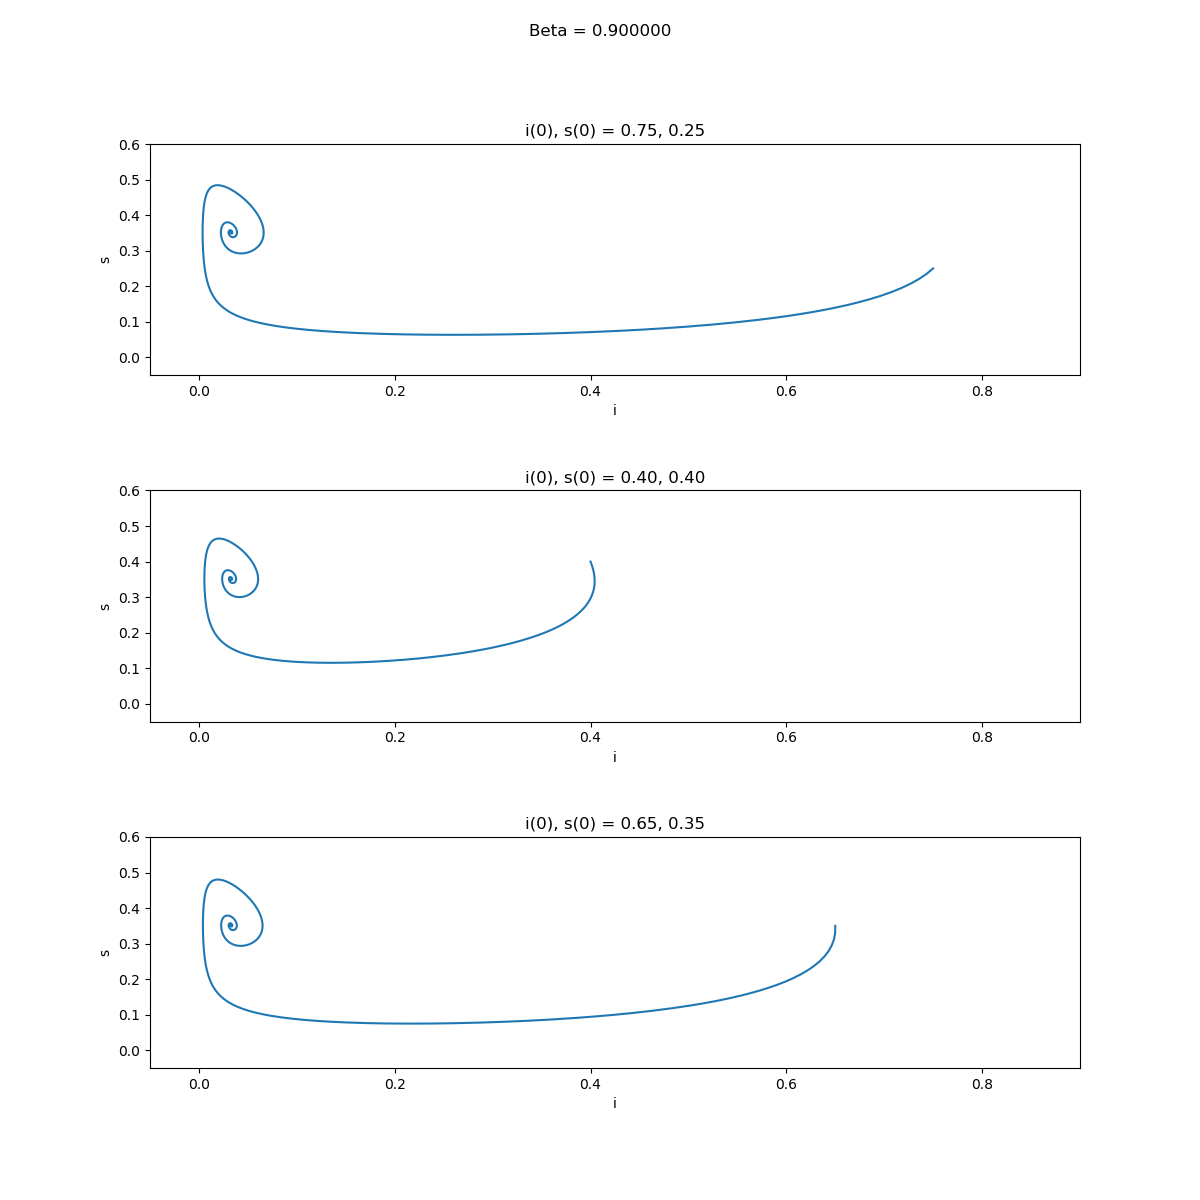
\includegraphics[width = 160mm]{Figures/Task1_0.png}
	\caption{}
	\label{fig:Task1_0}
\end{figure}
\begin{figure}[h!]
	\centering
	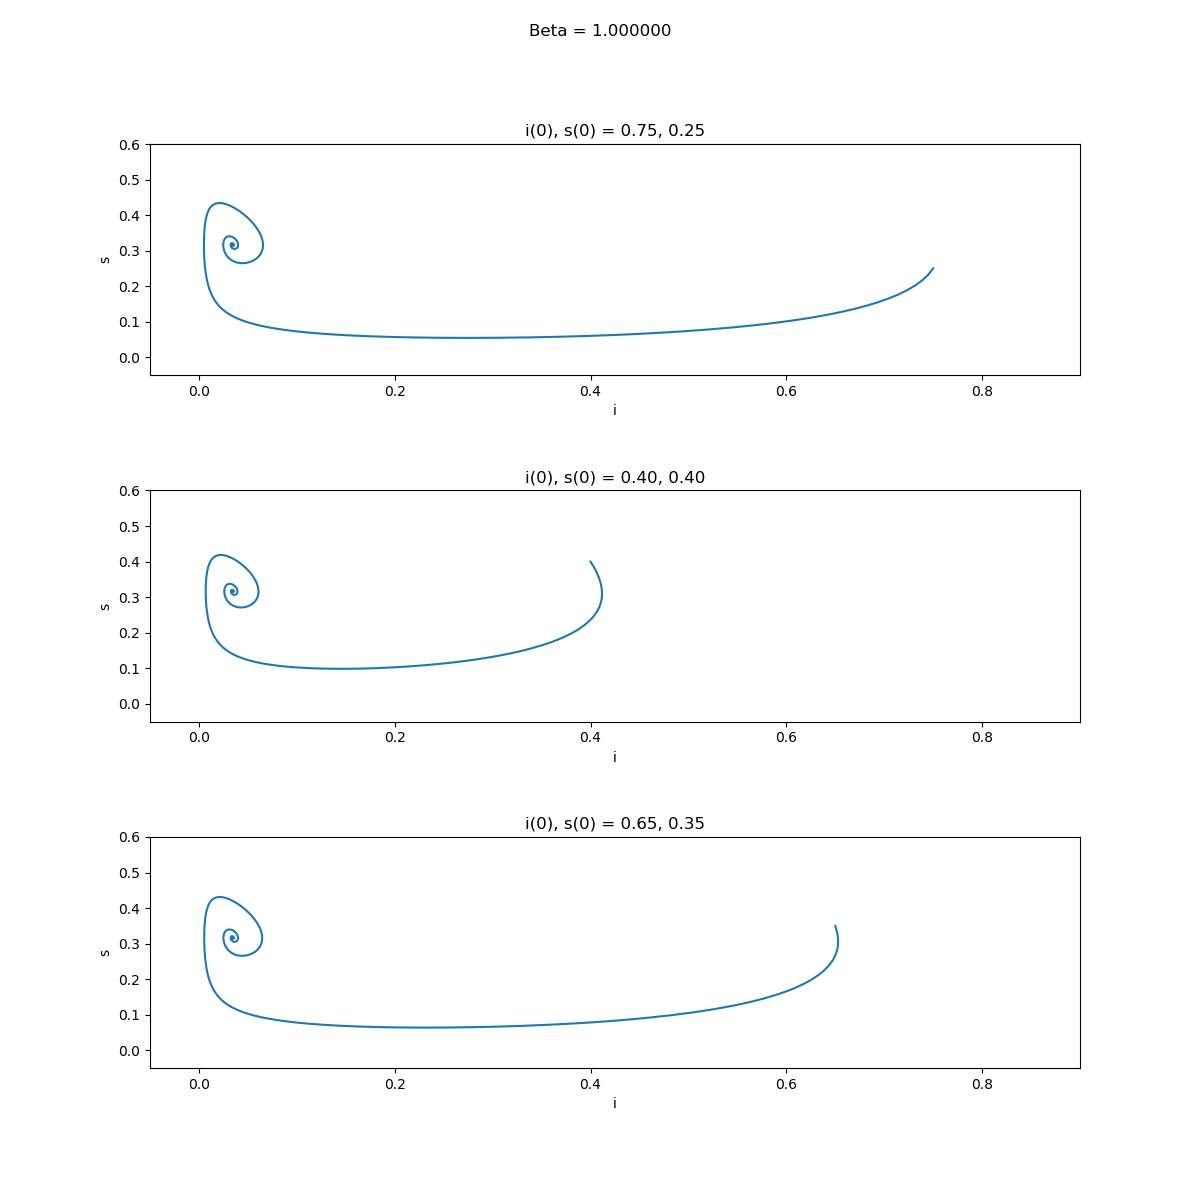
\includegraphics[width = 160mm]{Figures/Task1_1.png}
	\caption{}
	\label{fig:Task1_1}
\end{figure}

\begin{figure}[h!]
	\centering
	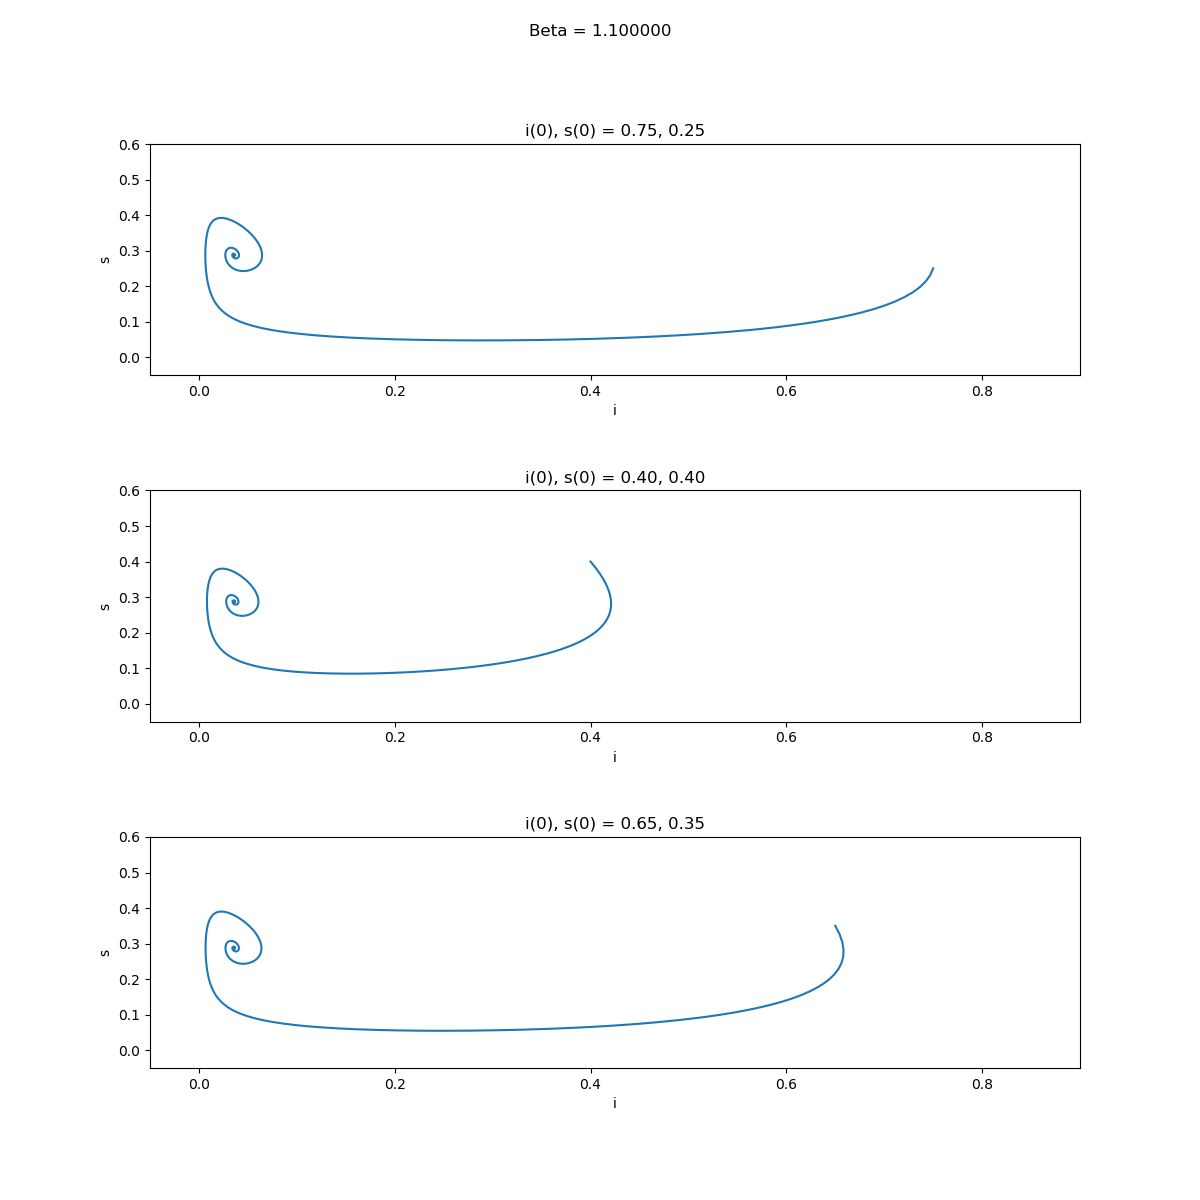
\includegraphics[width = 160mm]{Figures/Task1_2.png}
	\caption{}
	\label{fig:Task1_2}
\end{figure}

\begin{figure}[h!]
	\centering
	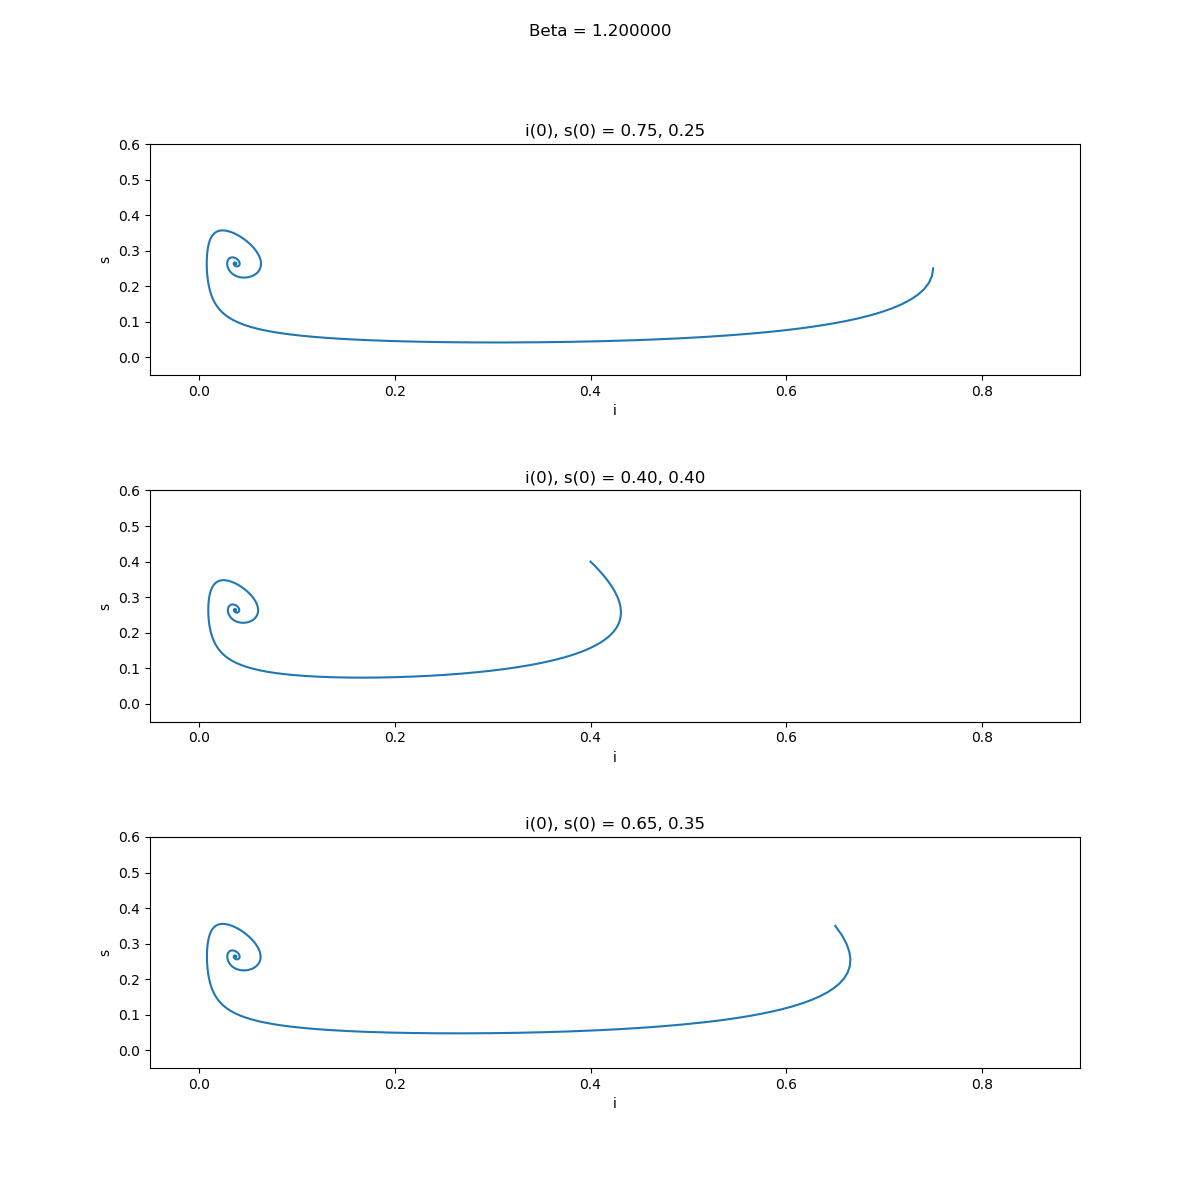
\includegraphics[width = 160mm]{Figures/Task1_3.png}
	\caption{}
	\label{fig:Task1_3}
\end{figure}

\begin{figure}[h!]
	\centering
	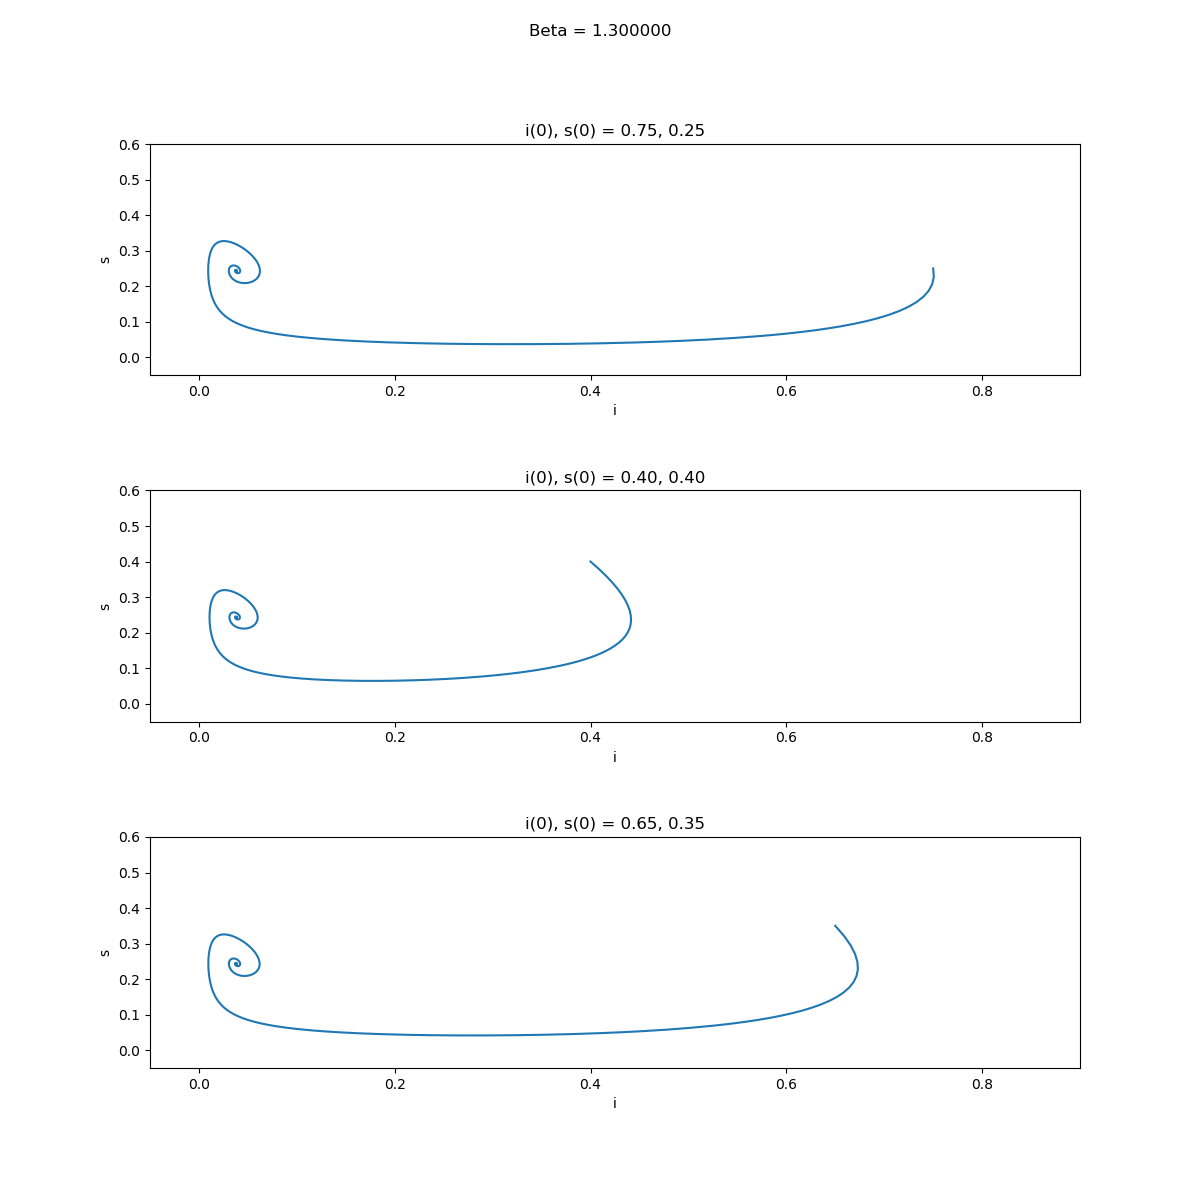
\includegraphics[width = 160mm]{Figures/Task1_4.png}
	\caption{}
	\label{fig:Task1_4}
\end{figure}

\begin{figure}[h!]
	\centering
	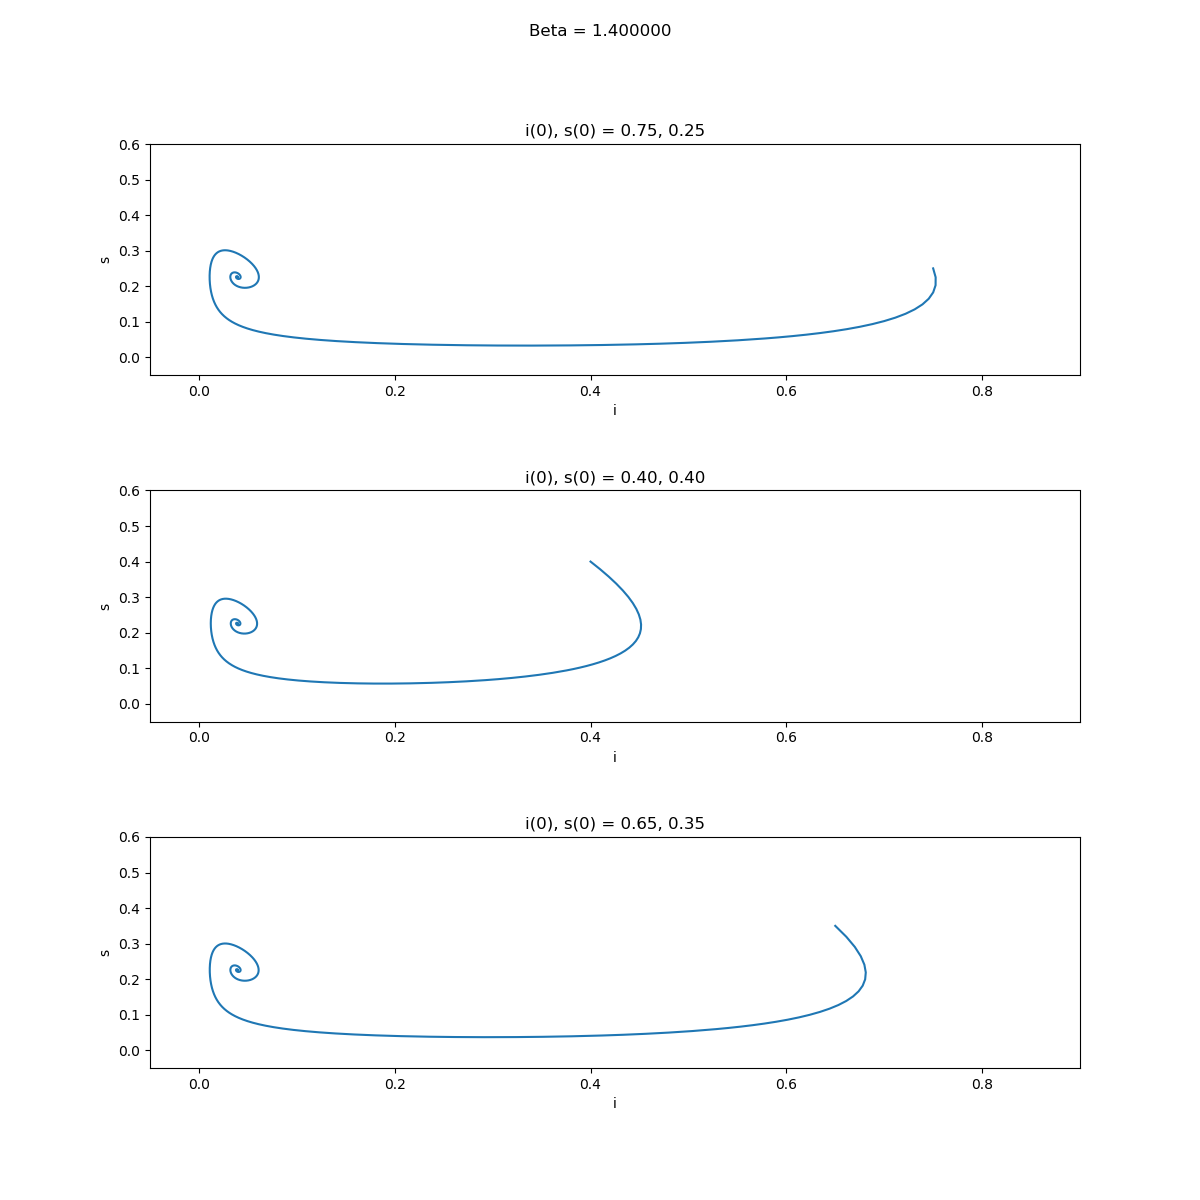
\includegraphics[width = 160mm]{Figures/Task1_5.png}
	\caption{}
	\label{fig:Task1_5}
\end{figure}

\begin{figure}[h!]
	\centering
	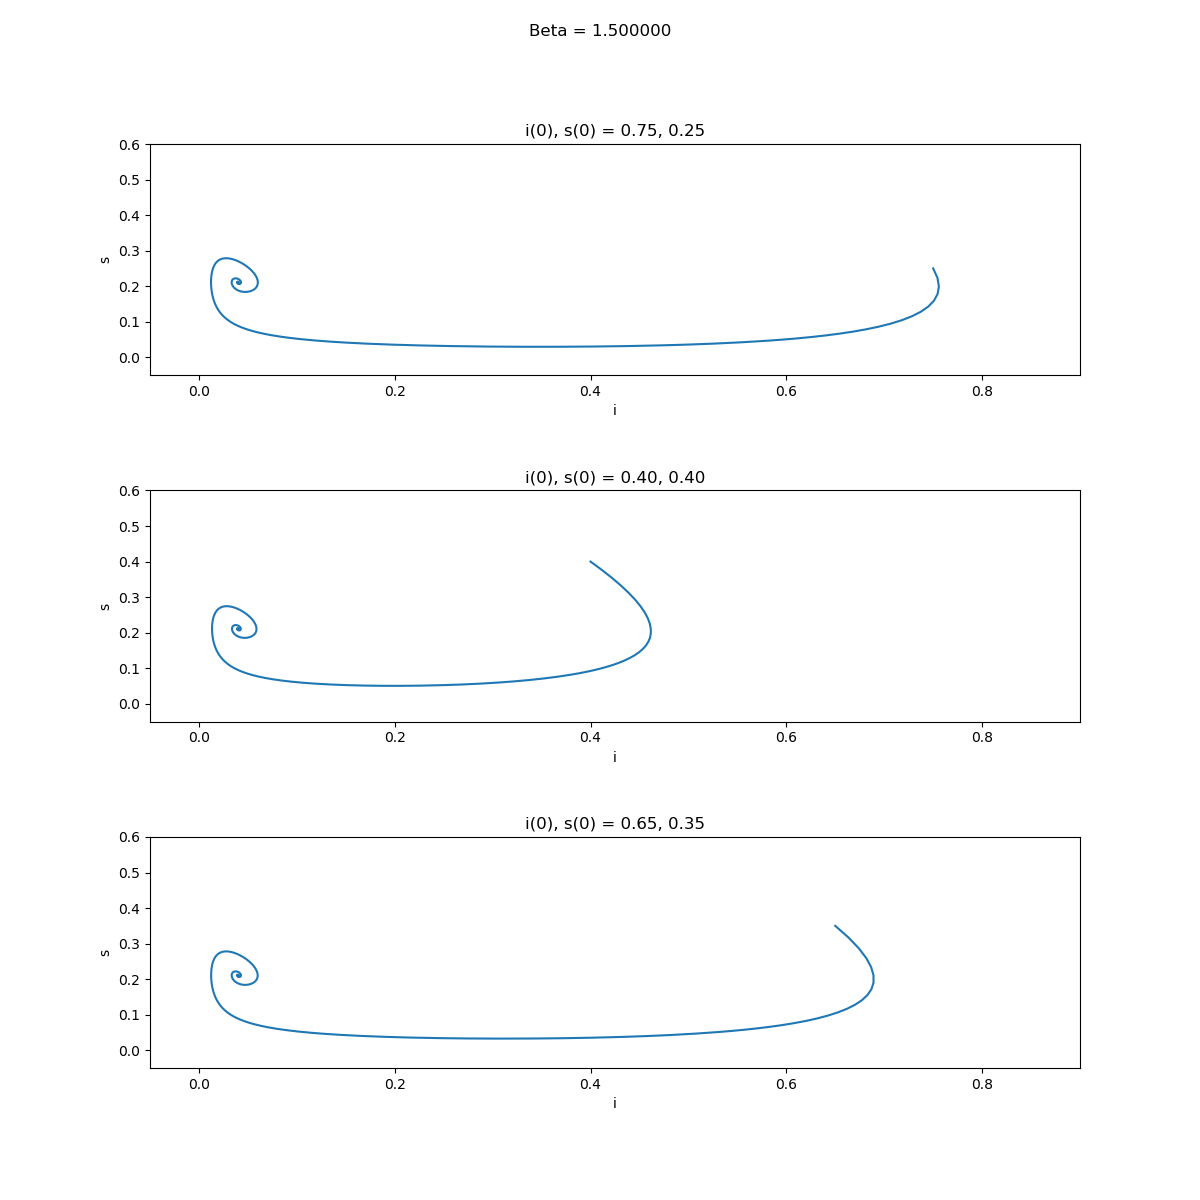
\includegraphics[width = 160mm]{Figures/Task1_6.png}
	\caption{}
	\label{fig:Task1_6}
\end{figure}





\clearpage
\subsection{Code}
\lstinputlisting[language=Python,style = PythonStyle]{Code/ComputationalTask2_Part1.py}
\newpage
\section{Mass action Law}
\subsection{Theory and Analysis}
\begin{gather}
\textrm{Mass action law equations} \notag \\	
\label{Eq:MAL1}
\gamma_{\rho i} = \beta_{\rho i} - \alpha_{\rho i} \\
\label{Eq:MAL2}
r_{\rho} = k_{\rho}\sum_{i = 1}^{n} c^{\alpha_{\rho i}} \\
\label{Eq:MAL3}
\frac{d\vec{c}}{dt} = \sum_{\rho}\gamma_{\rho}r_{\rho}
\end{gather}

\begin{gather}
\label{Reactions}
\textrm{Reactions} \notag \\
\ce{2Z <=> 2X} \\
\ce{Z <=> Y} \\
\ce{X + Y -> 2Z} \\
\ce{Z <=> Q} 
\end{gather}
Using Equations \eqref{Eq:MAL1},\eqref{Eq:MAL2} and \eqref{Eq:MAL3} and the knowledge that $x + y + q + z = 1$ we can find that the MAL equations for x,y and q are

\begin{gather}
\textrm{MAL Equations for above reactions} \notag \\
\frac{dX}{dt} = 2k_{1}Z^{2} - 2k_{-1}X^{2} - k_{3}XY \\
\frac{dY}{dt} = k_{2}Z - k_{-2}Y - k_{3}XY \\
\frac{dQ}{dt} = k_{4}Z - k_{-4}Q \\
\frac{dZ}{dt} = - 2k_{1}Z^{2} + 2k_{-1}X^{2} - k_{2}Z + k_{-2}Y + 2k_{3}XY -  k_{4}Z + k_{-4}Q 
\end{gather}
We can then use the above equations with the naive numerical method of the Euler method to numerically plot out the behaviour of $x(t),y(t),q(t)$


\newpage
\subsection{Graphs}
\begin{figure}[h!]
	\centering
	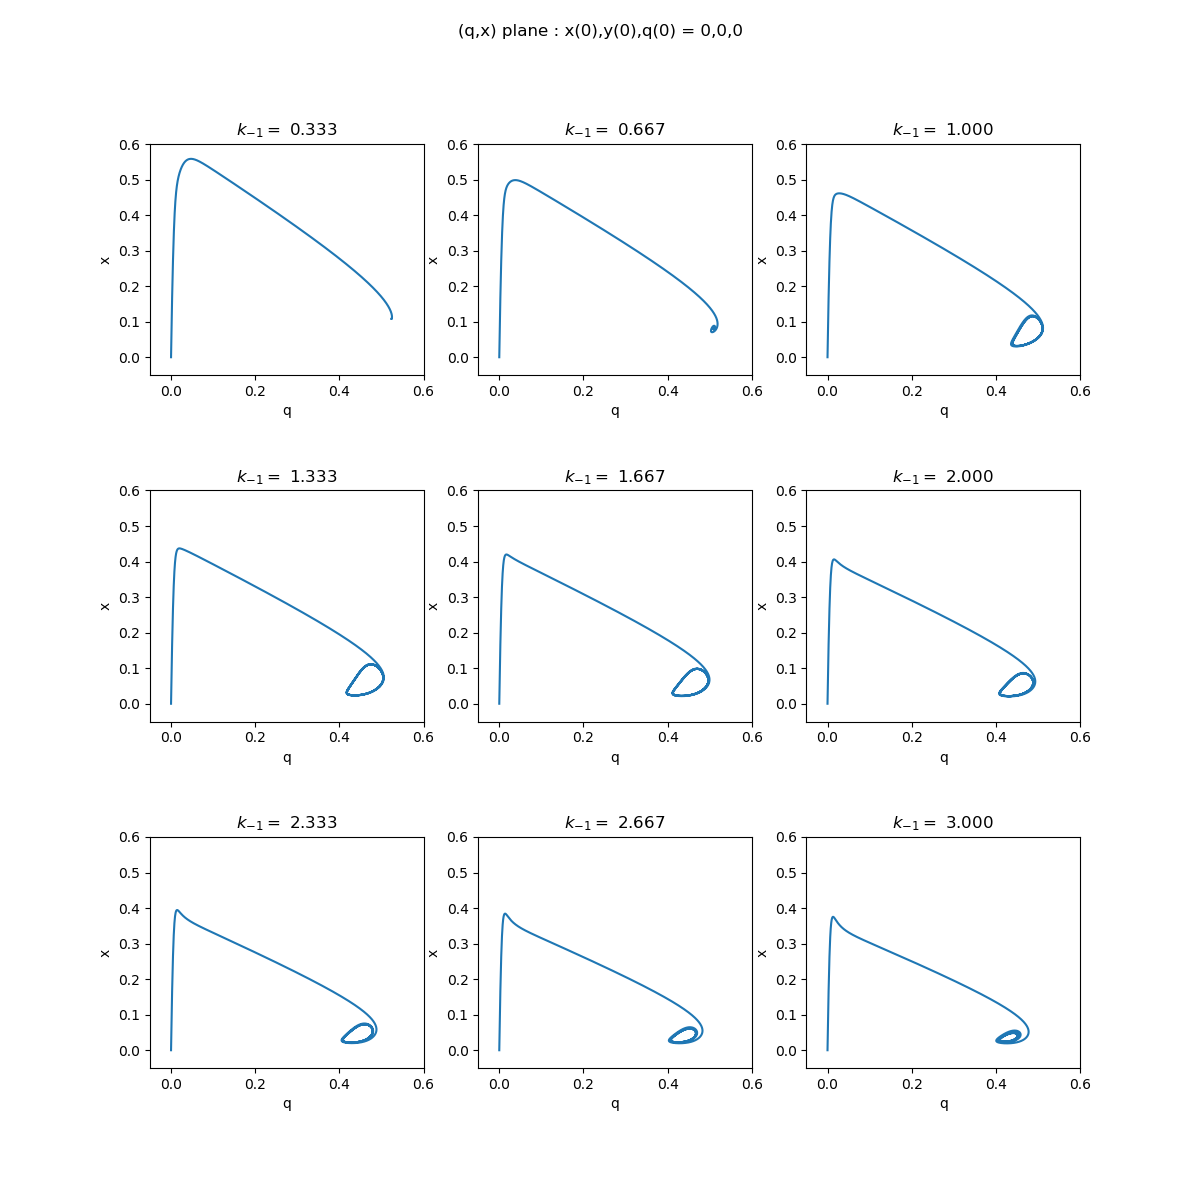
\includegraphics[width = 160mm]{Figures/Task2_1.png}
	\caption{For the initial conditions where $X(0),Y(0),Z(0) = 0,0,0$ plotting the X values against Q. As we can see in the plots for small $k_{-1}$ X rapidly increases then declines as Q increases while for larger $k_{-1}$ we can see that a periodic function is set up where the values for X and Q periodically repeat because of the oval we can see in this phase diagram. Also at larger $k_{-1}$, X initially in the transient phase does not increase as much as for smaller $k_{-1}$, which makes sense since larger $k_{-1}$ implies a faster reaction from 2X to 2Z, which then induces a faster increase in Q since it's concentration only depends on Z.}
	\label{fig:Task2_1}
\end{figure}


\begin{figure}[h!]
	\centering
	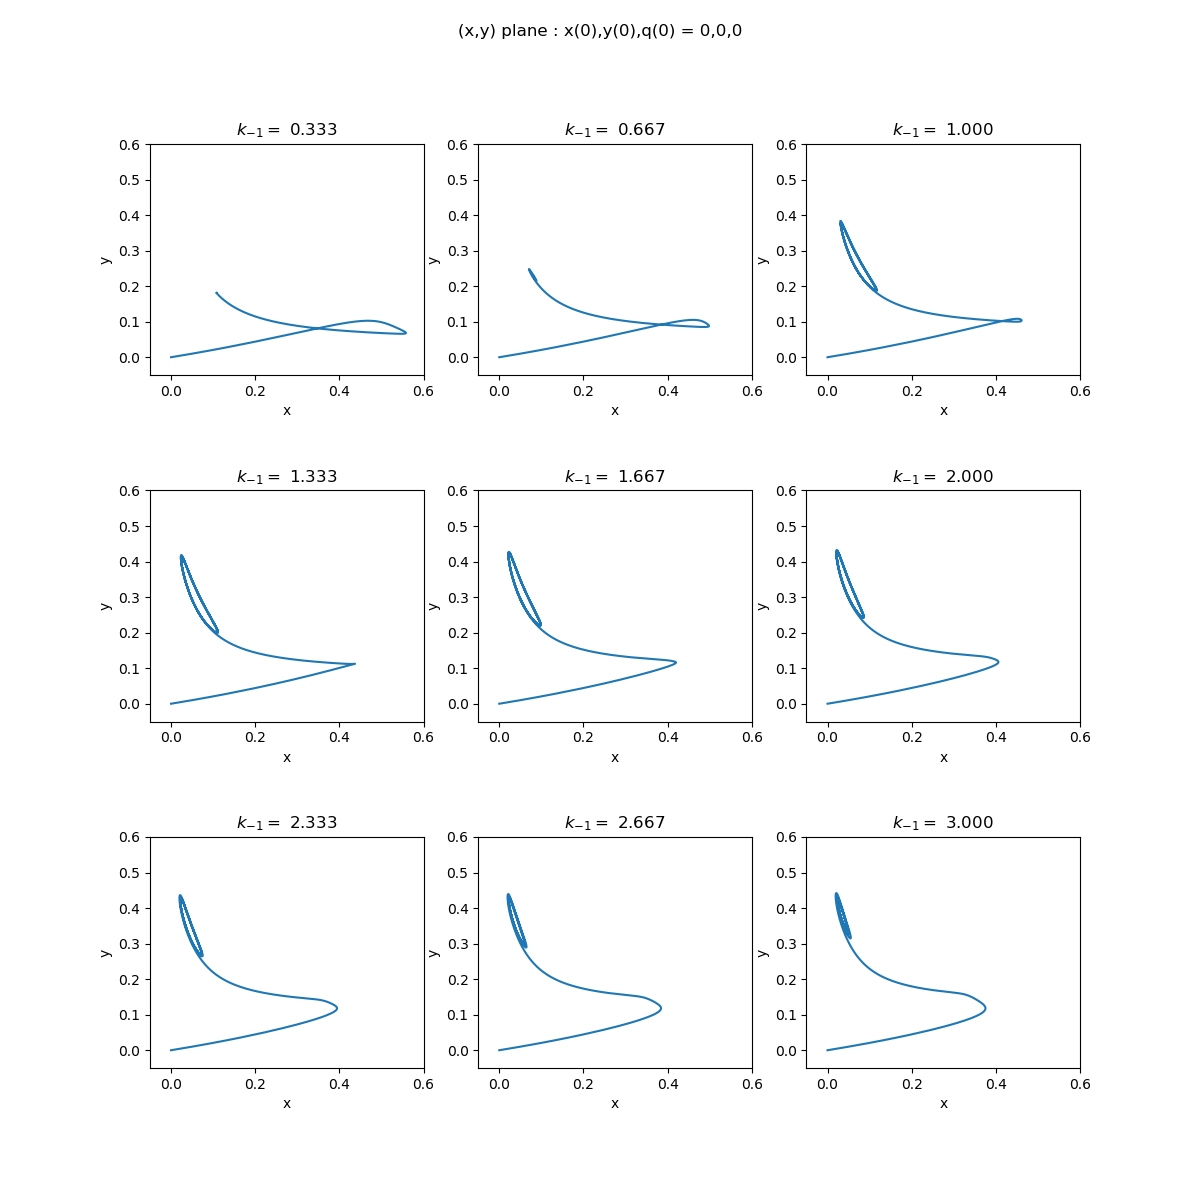
\includegraphics[width = 160mm]{Figures/Task2_2.png}
	\caption{For the initial conditions where $X(0),Y(0),Z(0) = 0,0,0$ plotting the Y values against X. The behaviour is more complicated in this graph. Since first X increases a lot with Y increasing only a little and then Y increases rapidly while X decreases rapidly. Again for smaller $k_{-1}$ the graph simply terminates at some point while for larger $k_{-1}$ we can see that the X and Y values become periodic as they move around the oval section. From this we can see that for larger $k_{-1}$ and Figure \ref{fig:Task2_1}} that the values for $X,Y,Q$ would start at the initial state and then move from a transient phase with less predictable behaviour into a steady state phase with very predictable concentration levels. 
	\label{fig:Task2_2}
\end{figure}

\begin{figure}[h!]
	\centering
	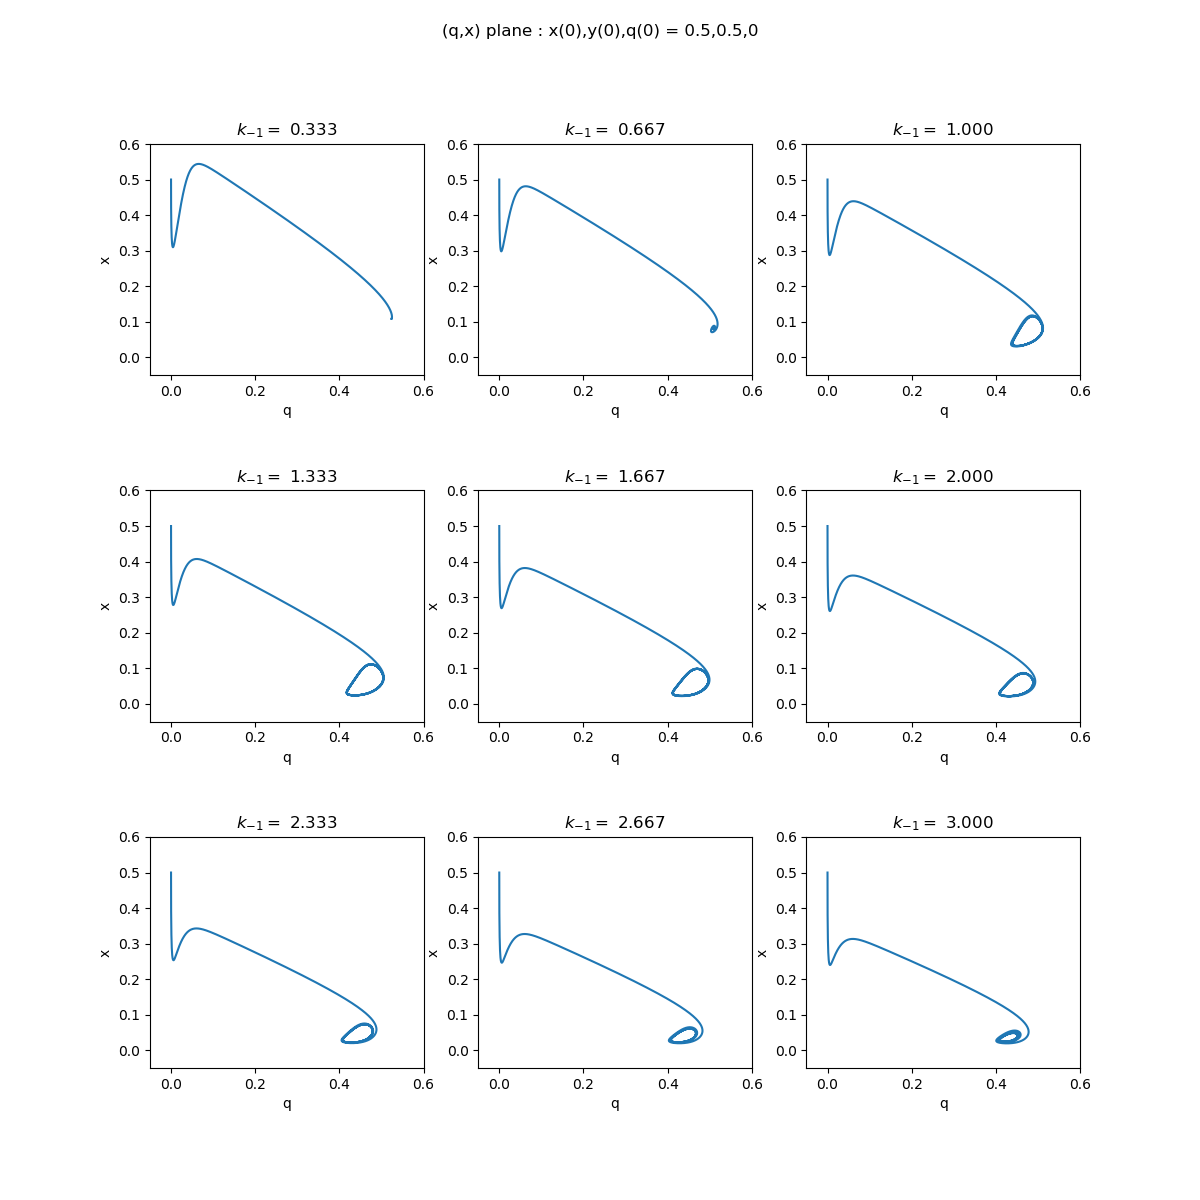
\includegraphics[width = 160mm]{Figures/Task2_3.png}
	\caption{For the initial conditions where $X(0),Y(0),Z(0) = 0.5,0.5,0$ plotting the X values against Q. As we can see when we compare these graphs to Figure \ref{fig:Task2_1}, the initial conditions affect the behaviour of the concentration levels in the initial transient phase drastically however both end up in the same region of the phase diagram in the same oval shape. Implying that their steady state behaviour is largely from what can be easily seen insensitive to the initial conditions and only depends on the functions themselves.   }
	\label{fig:Task2_3}
\end{figure}

\begin{figure}[h!]
	\centering
	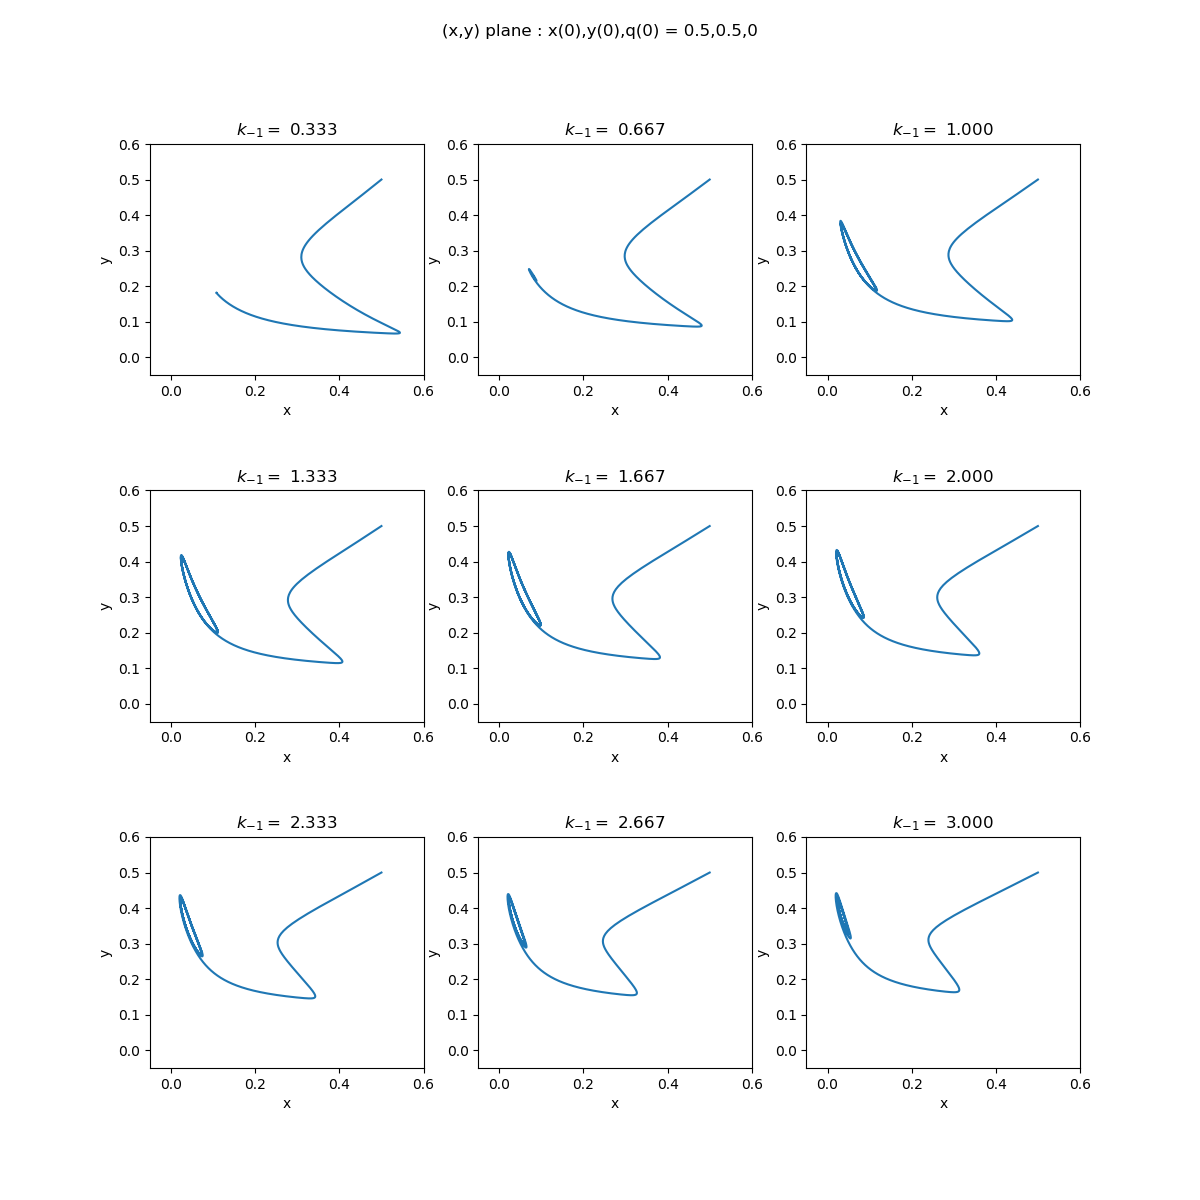
\includegraphics[width = 160mm]{Figures/Task2_4.png}
	\caption{For the initial conditions where $X(0),Y(0),Z(0) = 0.5,0.5,0$ plotting the Y values against X. As we can see when we compare these graphs to Figure \ref{fig:Task2_2}, the initial conditions affect the behaviour of the concentration levels in the initial transient phase drastically however both end up in the same region of the phase diagram in the same oval shape. Implying that their steady state behaviour is largely from what can be easily seen insensitive to the initial conditions and only depends on the functions themselves.}
	\label{fig:Task2_4}
\end{figure}


\clearpage
\subsection{Code}
\lstinputlisting[language=Python,style = PythonStyle]{Code/ComputationalTask2_Part2.py}



\newpage
\section{Lotka-Volterra}
\subsection{Theory and Analysis}

\begin{gather}
	\textrm{Lotka-Volterra Equations} \notag \\
	\label{Eq:LVE1}
	\frac{dx}{dt} = \alpha x - \beta xy \\
	\label{Eq:LVE2}
	\frac{dy}{dt} = \delta xy - \gamma y
\end{gather}

\begin{gather}
\textrm{Lotka-Volterra Equations with Logistic growth} \notag \\
\label{Eq:LVE1Log}
\frac{dx}{dt} = \alpha x(1 - Kx) - \beta xy \\
\label{Eq:LVE2Log}
\frac{dy}{dt} = \delta xy - \gamma y
\end{gather}

\newpage
\subsection{Graphs}
\begin{figure}[h!]
	\centering
	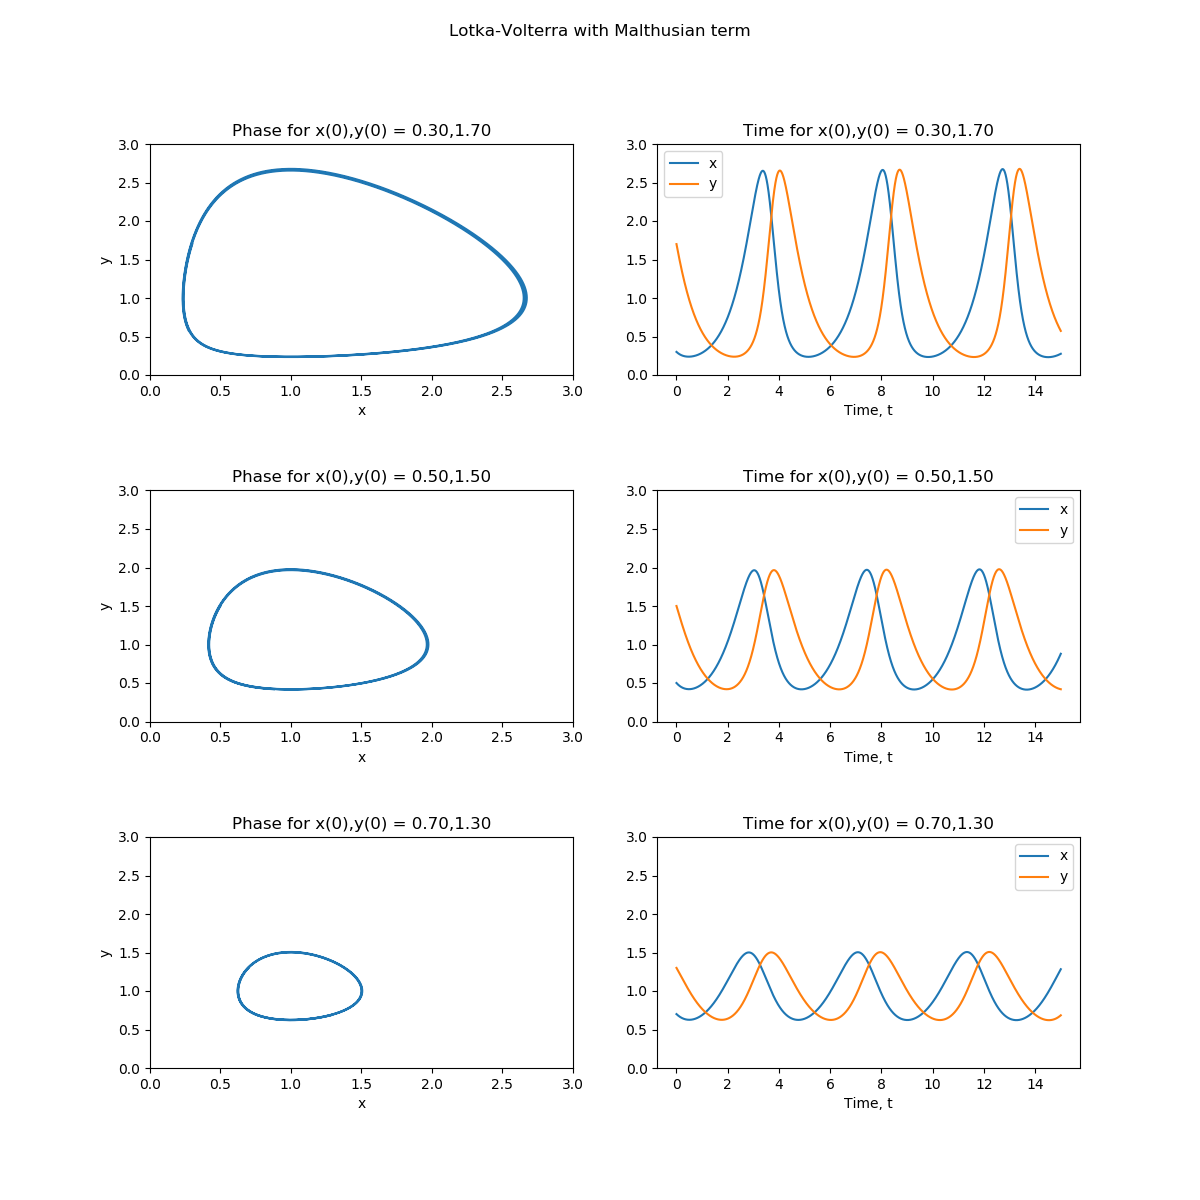
\includegraphics[width = 160mm]{Figures/Task3LV.png}
	\caption{In this figure we can clearly see that the results with a Malthusian term are periodic but is sensitive to the initial conditions. Effectively, the initial conditions regulate the amplitude of the sinusoidal function. The values for x trail the values for y because originally the Lotka-Volterra equations represented the relationship between predator and prey populations. In the case of predator and prey relations as the number of prey increases there is a time lag until the number of predators increase despite sufficient food due to pregnancy taking time etc. As the predator numbers then increase the number of prey falls as they get eaten by the predator, at which point after some delay due to fat reserves on the predator etc, the predators start to starve to death and their population collapses. At which point prey increases due to the lack of predators. And thus it continues in a cycle. The Lotka-Volterra equations do however assume that the prey always has enough food etc. Effectively, the predator and prey populations function like an undamped SHM.}
	\label{fig:Task3LV}
\end{figure}
\begin{figure}[h!]
	\centering
	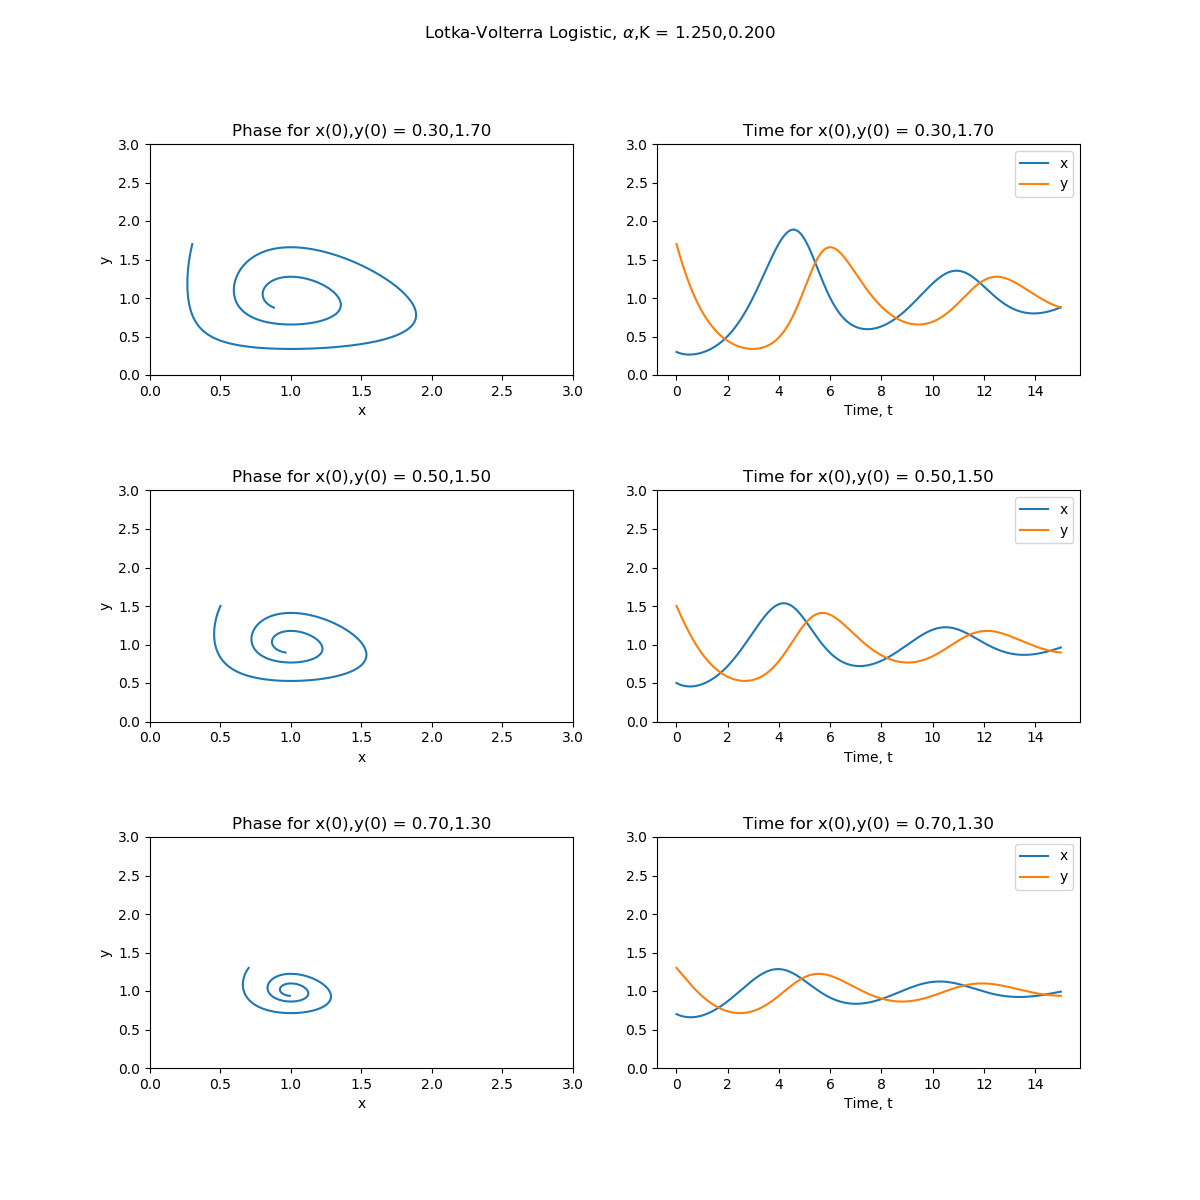
\includegraphics[width = 160mm]{Figures/Task3LLV0.png}
	\caption{In this figure we added logistic growth with $\alpha,K = 1.25,0.2$ where $\alpha$ is the growth rate and K is the carrying capacity. As we can see for these values of $\alpha,K$ the behaviour is still sinusoidal as in Figure \ref{fig:Task3LV} however the carrying capacity acts as a damping force meaning that as time goes on the difference between population highs and population lows reduces. This makes sense because every time the population of the prey species approaches the carrying capacity their growth slows and as their growth slows so does the prey species time lagged growth slow which in turn reduces the speed of population collapse of the prey due to not as high numbers of predators. However in this figure the periodicity does not stop it simply reduces in amplitude. i.e it functions as an underdamped SHM}
	\label{fig:Task3LLV0}
\end{figure}
\begin{figure}[h!]
	\centering
	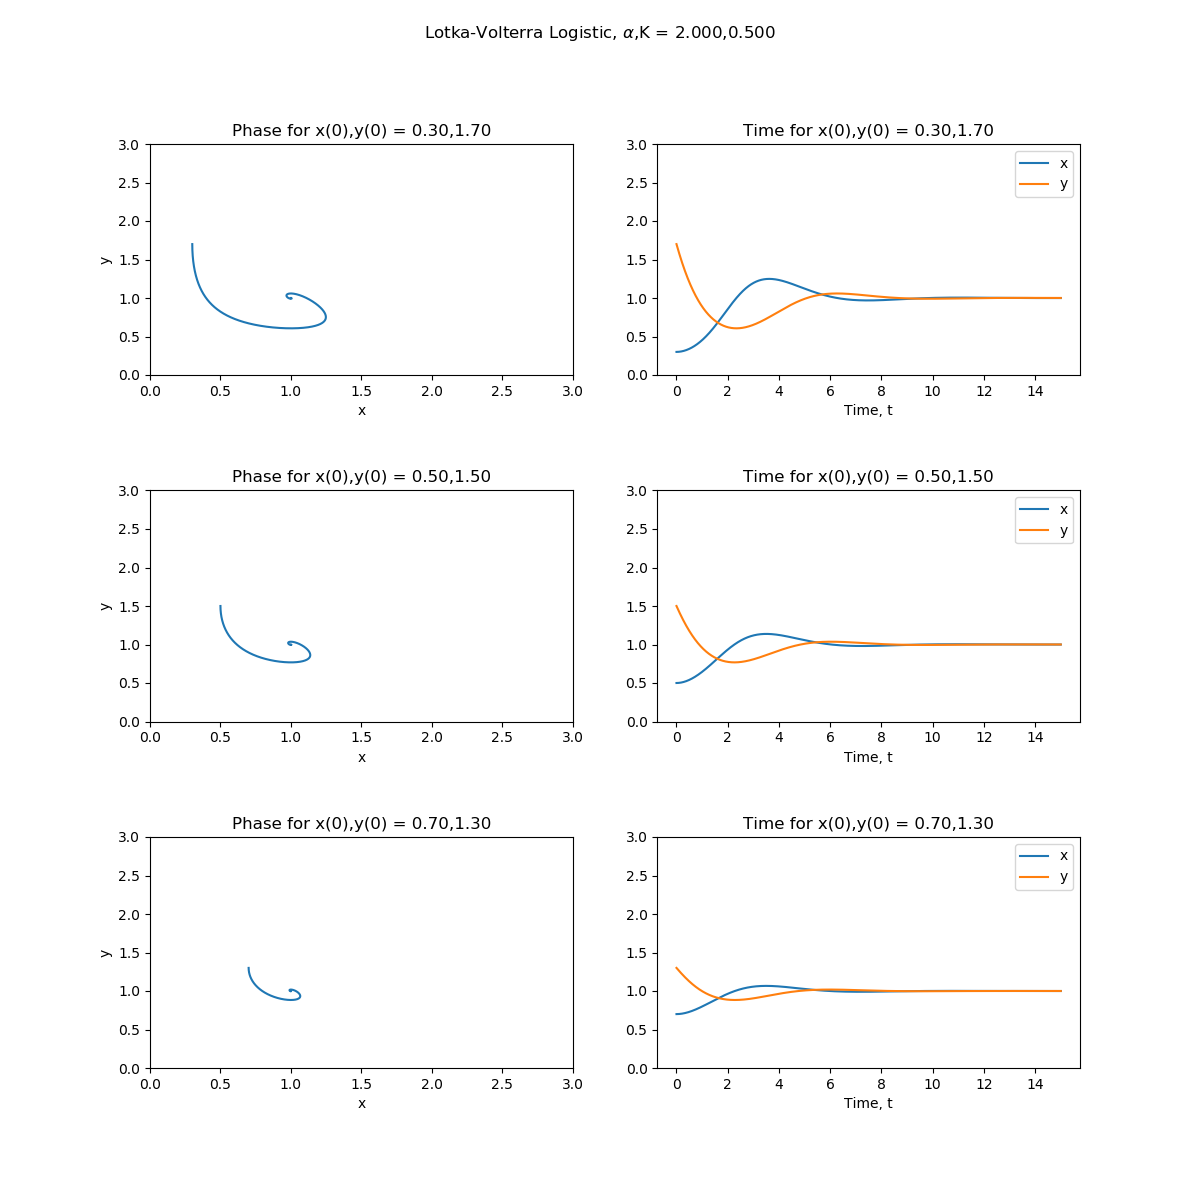
\includegraphics[width = 160mm]{Figures/Task3LLV1.png}
	\caption{In this figure like in Figure \ref{fig:Task3LLV0} the prey and population levels are underdamped however the damping factor is larger than in Figure \ref{fig:Task3LLV0} so it approaches the equilibrium level faster.}
	\label{fig:Task3LLV1}
\end{figure}
\begin{figure}[h!]
	\centering
	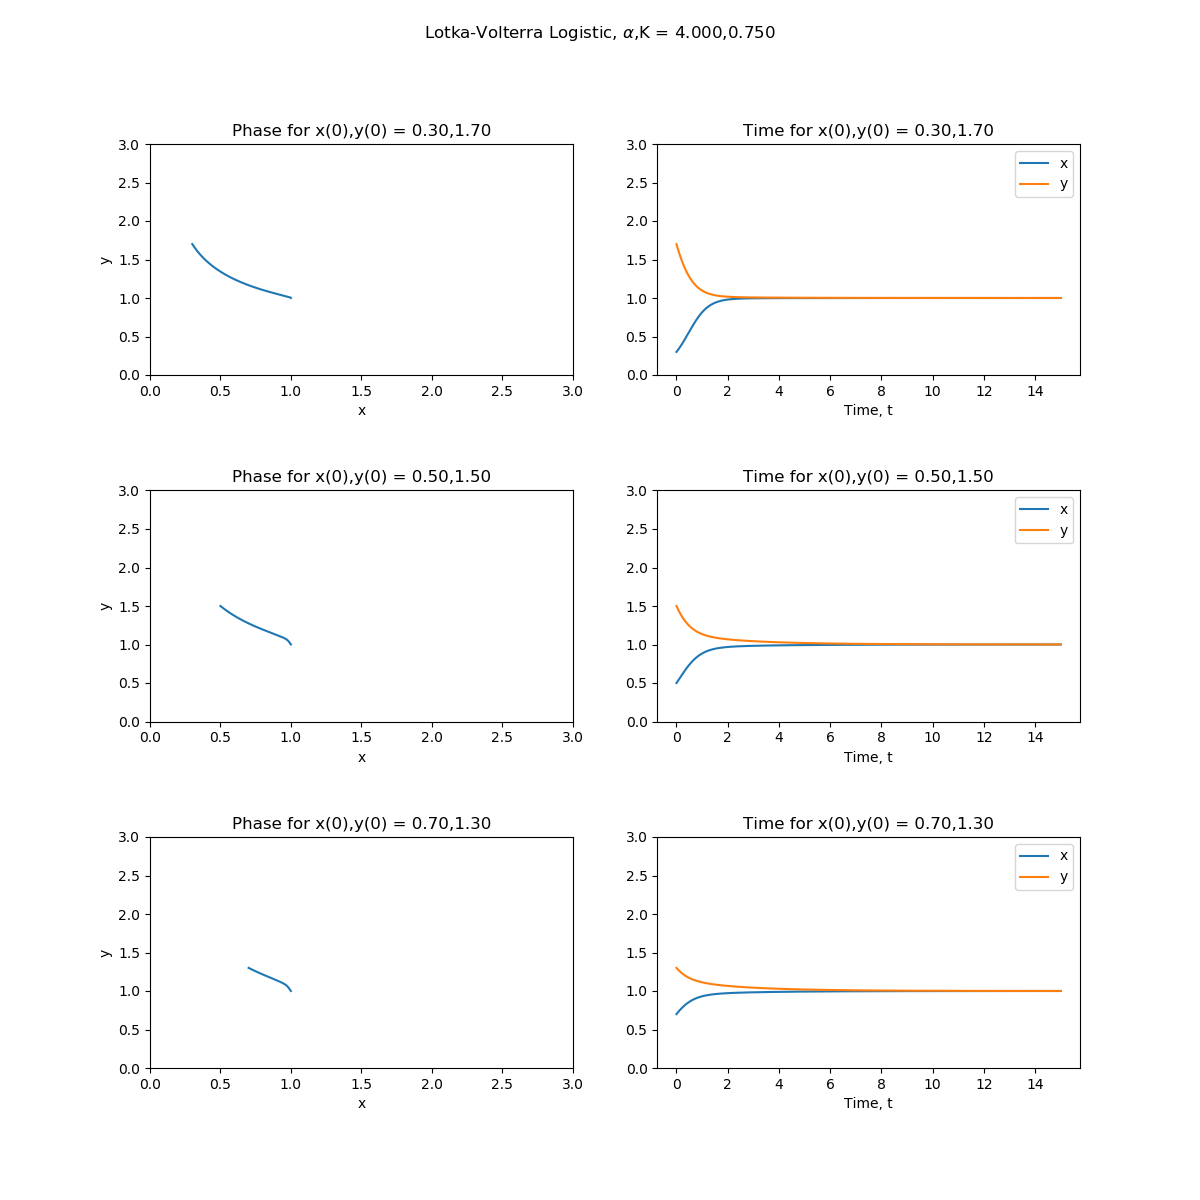
\includegraphics[width = 160mm]{Figures/Task3LLV2.png}
	\caption{In this figure the prey and population levels are critically damped so each population relaxes to the equilbrium level quickly. So this figure functions as a critically damped SHM.}
	\label{fig:Task3LLV2}
\end{figure}
\begin{figure}[h!]
	\centering
	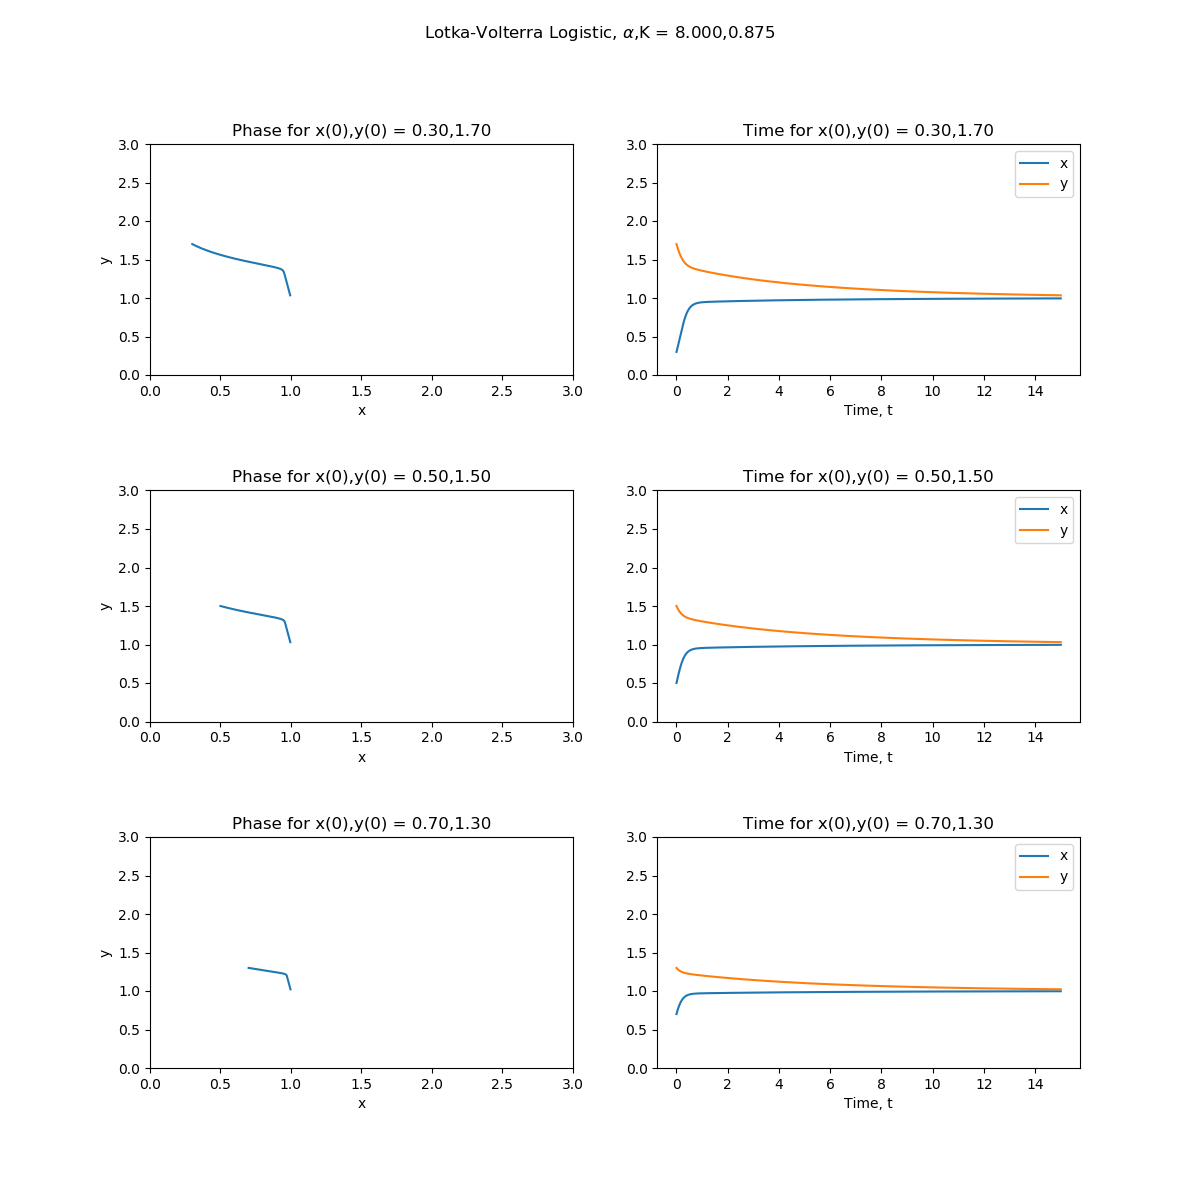
\includegraphics[width = 160mm]{Figures/Task3LLV3.png}
	\caption{In this figure the prey and population levels are over damped so each population relaxes to the equilbrium level slowly. So this figure functions as an overdamped SHM.}
	\label{fig:Task3LLV3}
\end{figure}
\clearpage

In all of the above Logistic Growth Lotka-Volterra Graphs(Figures \ref{fig:Task3LLV1},\ref{fig:Task3LLV2},\ref{fig:Task3LLV3}) we can see that the equilibrium value of the predator and prey species is insensitive to the initial conditions since it is always at x,y = 1. Overall the key takeaway from these plots is that firstly, ironically the predator population constantly chases the population level of the prey and that the carrying capacity i.e the environmental capability of supporting a certain amount of the prey acts as an important stabilizer of predator and prey population levels. And therefore the effects of changing the carrying capacity of the environment cause predictable population collapses or growths in both prey and predator species. 
\bigskip
Obviously, we could extend the Lotka-Volterra equations to be more realistic by chaining the predator and prey equations together such that we have multiple levels of species with each predating on the lower level while being the prey of the upper level. For example, Krill both eat Plankton and are eaten by Shrimps which are eaten by larger animals and so forth. 

\subsection{Code}
\lstinputlisting[language=Python,style = PythonStyle]{Code/ComputationalTask2_Part3.py}
\clearpage
\printmybibliography
\end{document}